\chapter{R}
	R is an integrated suite of software facilities for data manipulation, calculation and graphical
	display. \cite{venables2015introduction}
	\section{Basic commands}
	\subsection{Vectors}
	All the following implementations return a list of even numbers between 2 and 100
	\begin{lstlisting}[language=R]
		2*1:50
		seq(from=2, to=100, by=2)
		seq(from=2, length=50, by=2)
	\end{lstlisting}
		
	\subsection{Factors}
	\begin{lstlisting}[language=R]
		Create a list of names:
		names <- c("asd", ... , "asd")
		
		Encode the vector as factor:
		namef <- factor(names)
		
		Create a list of values of the same lenght of names:
		values <- c(1,2,3,...)
		
		Apply a function infolving boh arrays (e.g. the mean), values will be grouped accordingly with factors
		meanvalues <- tapply(values, names, mean)
	\end{lstlisting}

	
	\subsection{Functions}
	A function can be built in a simple way:
	\begin{lstlisting}[language=R]
	stderr <- function(x) sqrt(var(x)/length(x))
	incster <- tapply(values, namef, stderr)
	\end{lstlisting}
	
	\subsection{Types}
	\subsubsection{Array}
	\begin{lstlisting}[language=R]
	A <-(data_vector, size)
	\end{lstlisting}
	
	\subsubsection{MatrixIX}
	http://www.r-tutor.com/r-introduction/matrix
	A = matrix(c(2,3,4,5,6,7,8,9,0), nrow=3, ncol=3, byrow = TRUE)
	product: $A \%*\% A$
	\begin{lstlisting}[language=R]
		A = matrix(c(2,3,4,5,6,7,8,9,0), nrow=3, ncol=3, byrow = TRUE)
		$A \%*\% A$	#product
		cbin() 		#Add column
		rbind() 	#Add row
	\end{lstlisting}
	
	\subsubsection{List}
	lst = list(reference="value", reference2=number, refererence3=c(1,2,3))

	to print a value:
	lst[[index]]
	lst\$reference

	to access a subvalue of a index/reference (e.g. the array) use 
	ls[[indexLst]][indexArray]

	a list can be attached attach(list) or detached detach(list). This makes the inner arguments of the list accessible as standard varaibles.
	
	\subsubsection{DataFrames}
	\hl{http://www.r-tutor.com/r-introduction/data-frame}
	
	A data frame is used for storing data tables. It is a list of vectors of equal length. For example, the following variable df is a data frame containing three vectors n, s, b.
	
	\subsection{Reading data from file}
	file="file\_name" can be omitted and a "file\_name" is used by default. The file has to be in the working direcotory

	\subsubsection{CSV}
	Data are separated by a comma, the first line is automatically recognized as a header
	\begin{lstlisting}[language=R]
		c = read.csv("input.csv")
	\end{lstlisting}
	
	\subsubsection{Table}
	Data are separate b whitespace, the first line will be used as header
	\begin{lstlisting}[language=R]
		t = read.table("input.dat", header = TRUE)
	\end{lstlisting}
	

	Useful additional arguments are:
	\begin{itemize}
	\itembf{sep = "separator\_char"}	e.g. sep = "\t" allows the usage of spaces into a table
	\itembf{na.strings = "string\_as\_na"} specify the char value corresponding tp NA in the table (e.g "-")
	\itembf{fill = TRUE}insert an empty value for empty rows but will left shift values in tables
	\end{itemize}
	
	\subsubsection{Scan}
	Scan("filename", what="type") interpred a file like a vector disregarding break line
	
	\subsection{Control Statements}
	\begin{lstlisting}[language=R]
		if(condition){
			...	
		}
		else {
			...
		}
	\end{lstlisting}
	
	\begin{lstlisting}[language=R]
		for(i in 1:n){
			...	
		}
	\end{lstlisting}
	
	\subsection{Data Conversion}
	Apply can be used to execute (apply) a fuction over a dataset. It has several variants, here the most useful:
	\begin{itemize}
		\itembf{apply} When you want to apply a function to the rows or columns of a matrix (and higher-dimensional analogues).
		\itembf{lapply} When you want to apply a function to each element of a list in turn and get a list back.
		\itembf{sapply} When you want to apply a function to each element of a list in turn, but you want a vector back, rather than a list.
		\itembf{tapply} For when you want to apply a function to subsets of a vector and the subsets are defined by some other vector, usually a factor.
	\end{itemize}
	
\section{Autogenerated Testcases Efficiency and Effectiveness}
	This section will re-analyze data collected during the experiment about Randoop auto-generated test cases respect to manual test cases. The esperiment involves several additional parameters:
	\begin{itemize}
		\itembf{System:} The source code to debug (xml-security or jtopas), one code can be more difficult to debug than the other.
		\itembf{Treatement:} Manual or Auto-generated test cases
		\itembf{Lab:} First or second session, may cause some learning effect.
		\itembf{Experience:} bachelor or master degree (bsc, msc)
		\itembf{Ability:} level of ability based on test and previous experiences (low, medium, high)
	\end{itemize}
	 Additional details can be found in the specific chapter.
	 
	 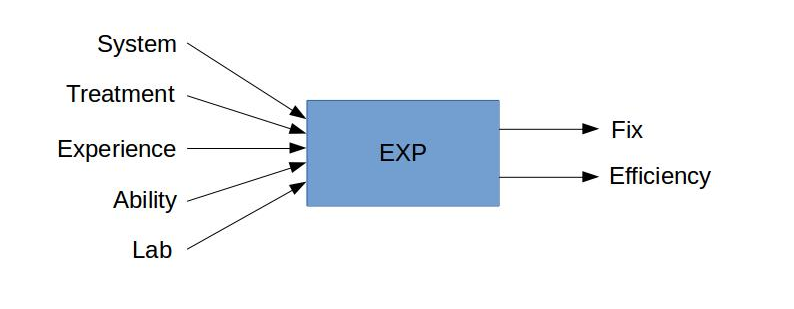
\includegraphics[ width=1 \linewidth]{./img/GLM_debugging.png}
	 As can be seen from the image the GLM considers parameters listed above and provides an estimation about Effectiveness (number of correctly fixed bugs) and Efficiency (time requested to fix a bug).
	 
\subsection{Script} \newpage
\begin{lstlisting}[language=R]
data = read.csv2("all.csv", sep=";", dec=",", header=TRUE)

# Delete useless rows
selected = data[,c("ID", "Experiment", "Group", "System", "Treatment", "Lab", "Experience", "Ability", "Time1", "Fix1", "Time2", "Fix2", "Time3", "Fix3", "Time4", "Fix4")]

# Selecting only "All" rows
all = selected[selected$Experiment == "All",]

# Generate the column "Fix"
sumna = function(a) sum(a, na.rm=TRUE)
all = cbind(all, apply(all[,c("Fix1", "Fix2", "Fix3", "Fix4")], 1, sumna)) 
colnames(all)[length(all)] = "Fix"

# Calculate efficiency, NA and NaN are converted to 0.
efficiency = function(a) if (a[9] != 0 )a[9]/sumna(c(a[1]*a[2], a[3], a[4], a[5]*a[6], a[7]*a[8])) else 0
alleff = cbind(all, apply(all[,c("Time1", "Fix1", "Time2", "Fix2", "Time3", "Fix3", "Time4", "Fix4", "Fix")], 1, efficiency)) 
colnames(alleff)[length(alleff)] = "Efficiency"

attach(alleff)
#Rename litteral data to integers 
abLevel = function(l) if(l == "low") 1 else if(l == "medium") 2 else if(l == "high") 3
Ability = sapply(alleff$Ability, abLevel)

#GLM
fixModel = glm(Fix ~ System + Treatment + Lab + Experience + Ability)
effModel = glm(Efficiency ~ System + Treatment + Lab + Experience + Ability)

#Draw effectiveness plots
boxplot(Fix ~ Ability, names=c("Low", "Medium", "High"), xlab="Ability", ylab="Effectiveness")
boxplot(Fix ~ Treatment, xlab="Treatment", ylab="Effectiveness")
interaction.plot(Treatment, alleff$Ability , Fix, trace.label = "Ability")

#Draw efficiency plot
interaction.plot(Treatment, Ability, names=c("Low", "Medium", "High"), Efficiency)
interaction.plot(Treatment, alleff$Ability , Efficiency)
interaction.plot(Treatment, alleff$Ability , Efficiency, trace.label = "Ability")

detach(allef)

\end{lstlisting}
	
\newpage
	\subsection{Effectiveness Results}
This is the raw data output of the effectiveness experiment's GLM.
\begin{lstlisting}[language=]
Call:
glm(formula = Fix ~ System + Treatment + Lab + Experience + Ability)

Deviance Residuals: 
 Min       1Q   Median       3Q      Max  
-1.5491  -0.7680  -0.2572   0.9079   2.2216  

Coefficients:
                Estimate Std. Error t value Pr(>|t|)    
(Intercept)         -1.3959     0.5404  -2.583 0.013195 *  
Systemxml-security  -0.2230     0.3050  -0.731 0.468539    
Treatmentrandom      0.6964     0.3036   2.294 0.026621 *  
Lablab2              0.2858     0.3126   0.914 0.365525    
Experiencemsc        0.7706     0.3193   2.413 0.020035 *  
Ability              0.9443     0.2579   3.661 0.000671 ***
---
Signif. codes:  0 ‘***’ 0.001 ‘**’ 0.01 ‘*’ 0.05 ‘.’ 0.1 ‘ ’ 1

(Dispersion parameter for gaussian family taken to be 1.133588)

 Null deviance: 93.380  on 49  degrees of freedom
Residual deviance: 49.878  on 44  degrees of freedom
AIC: 155.77

Number of Fisher Scoring iterations: 2
\end{lstlisting}

\begin{figure}
		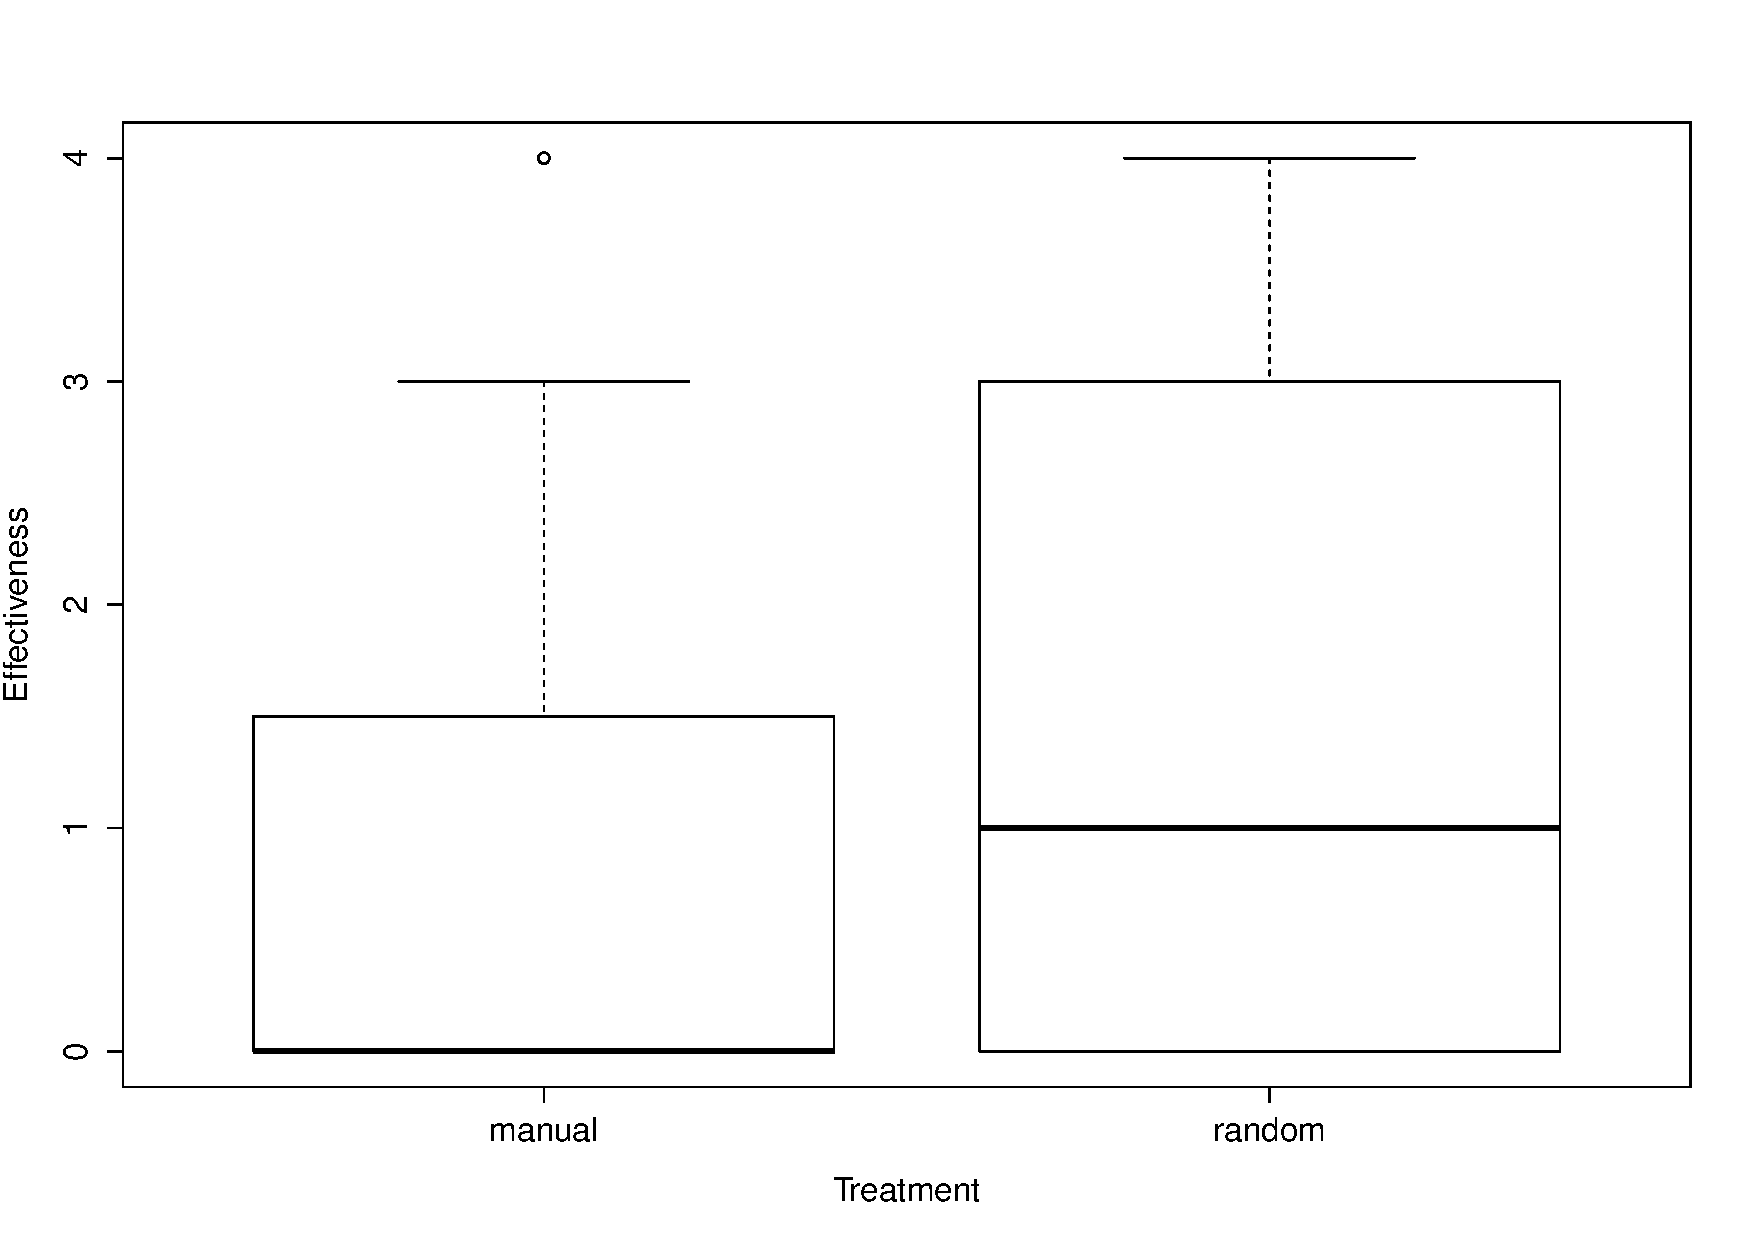
\includegraphics[ width=0.5 \linewidth]{./img/box_fix_treatment.pdf}
		\caption{Fix-Treatment Boxplot}
		\label{box_fix_treatment}
	\end{figure}

\begin{figure}
	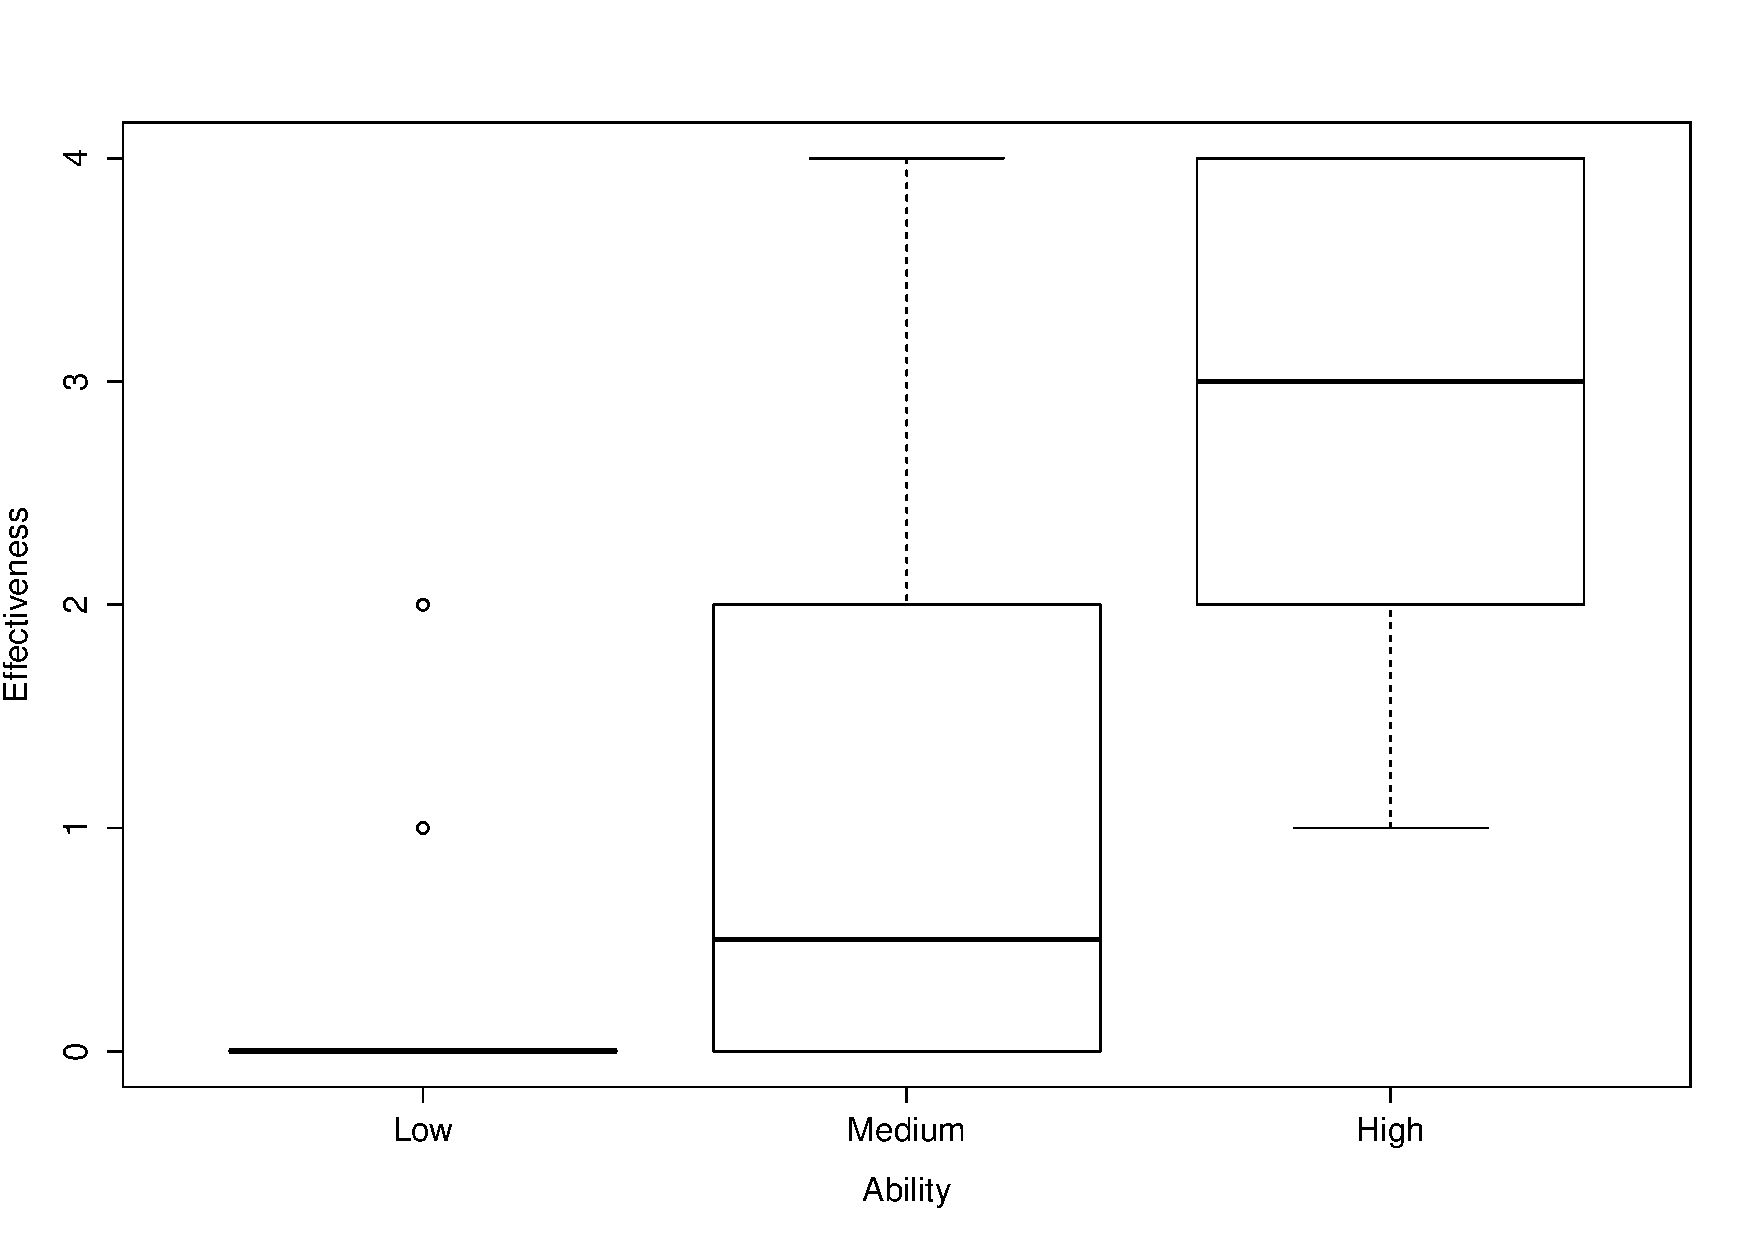
\includegraphics[ width=0.5 \linewidth]{./img/box_fix_ability.pdf}
	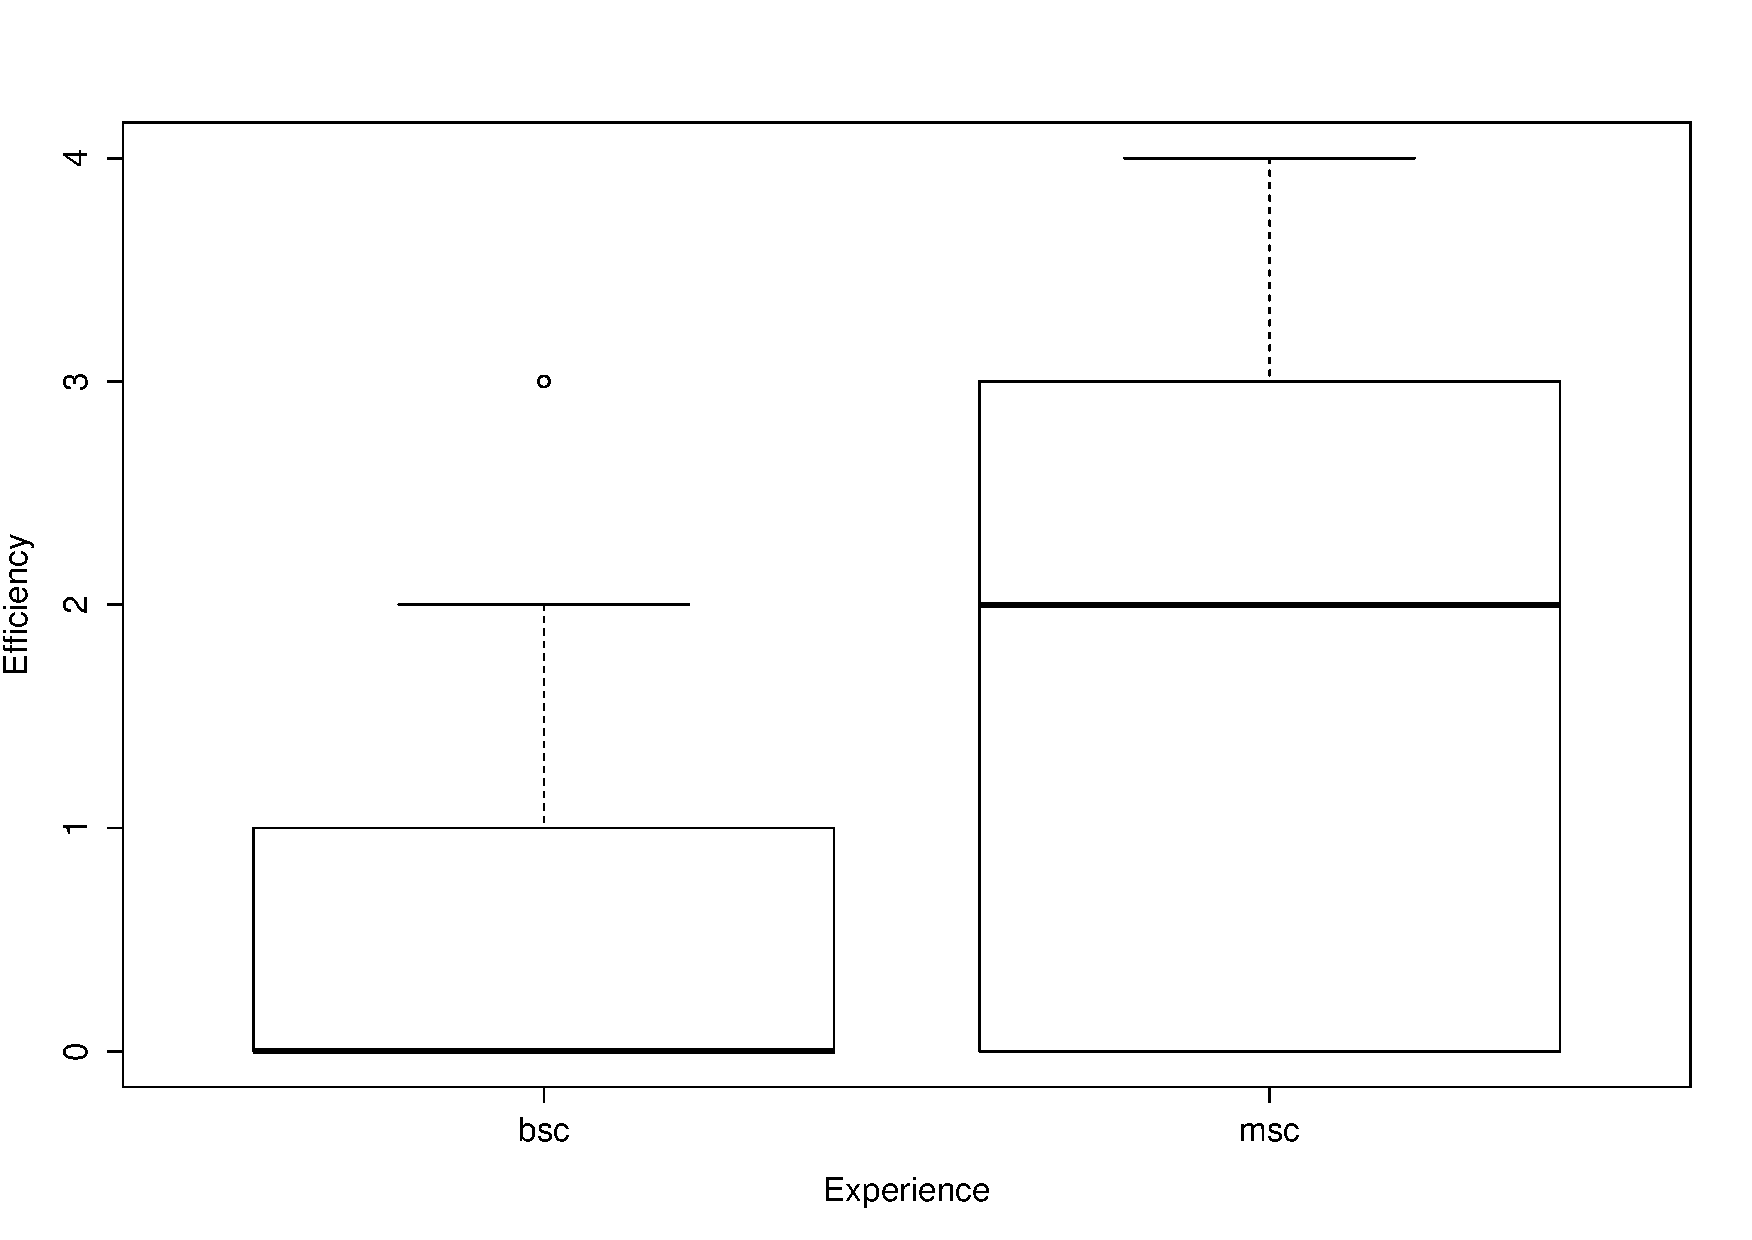
\includegraphics[ width=0.5 \linewidth]{./img/box_fix_experience.pdf}
	\caption{Effectiveness respect to Ability and experience Boxplots}
	\label{box_fix_ability}
\end{figure}

\begin{figure}
	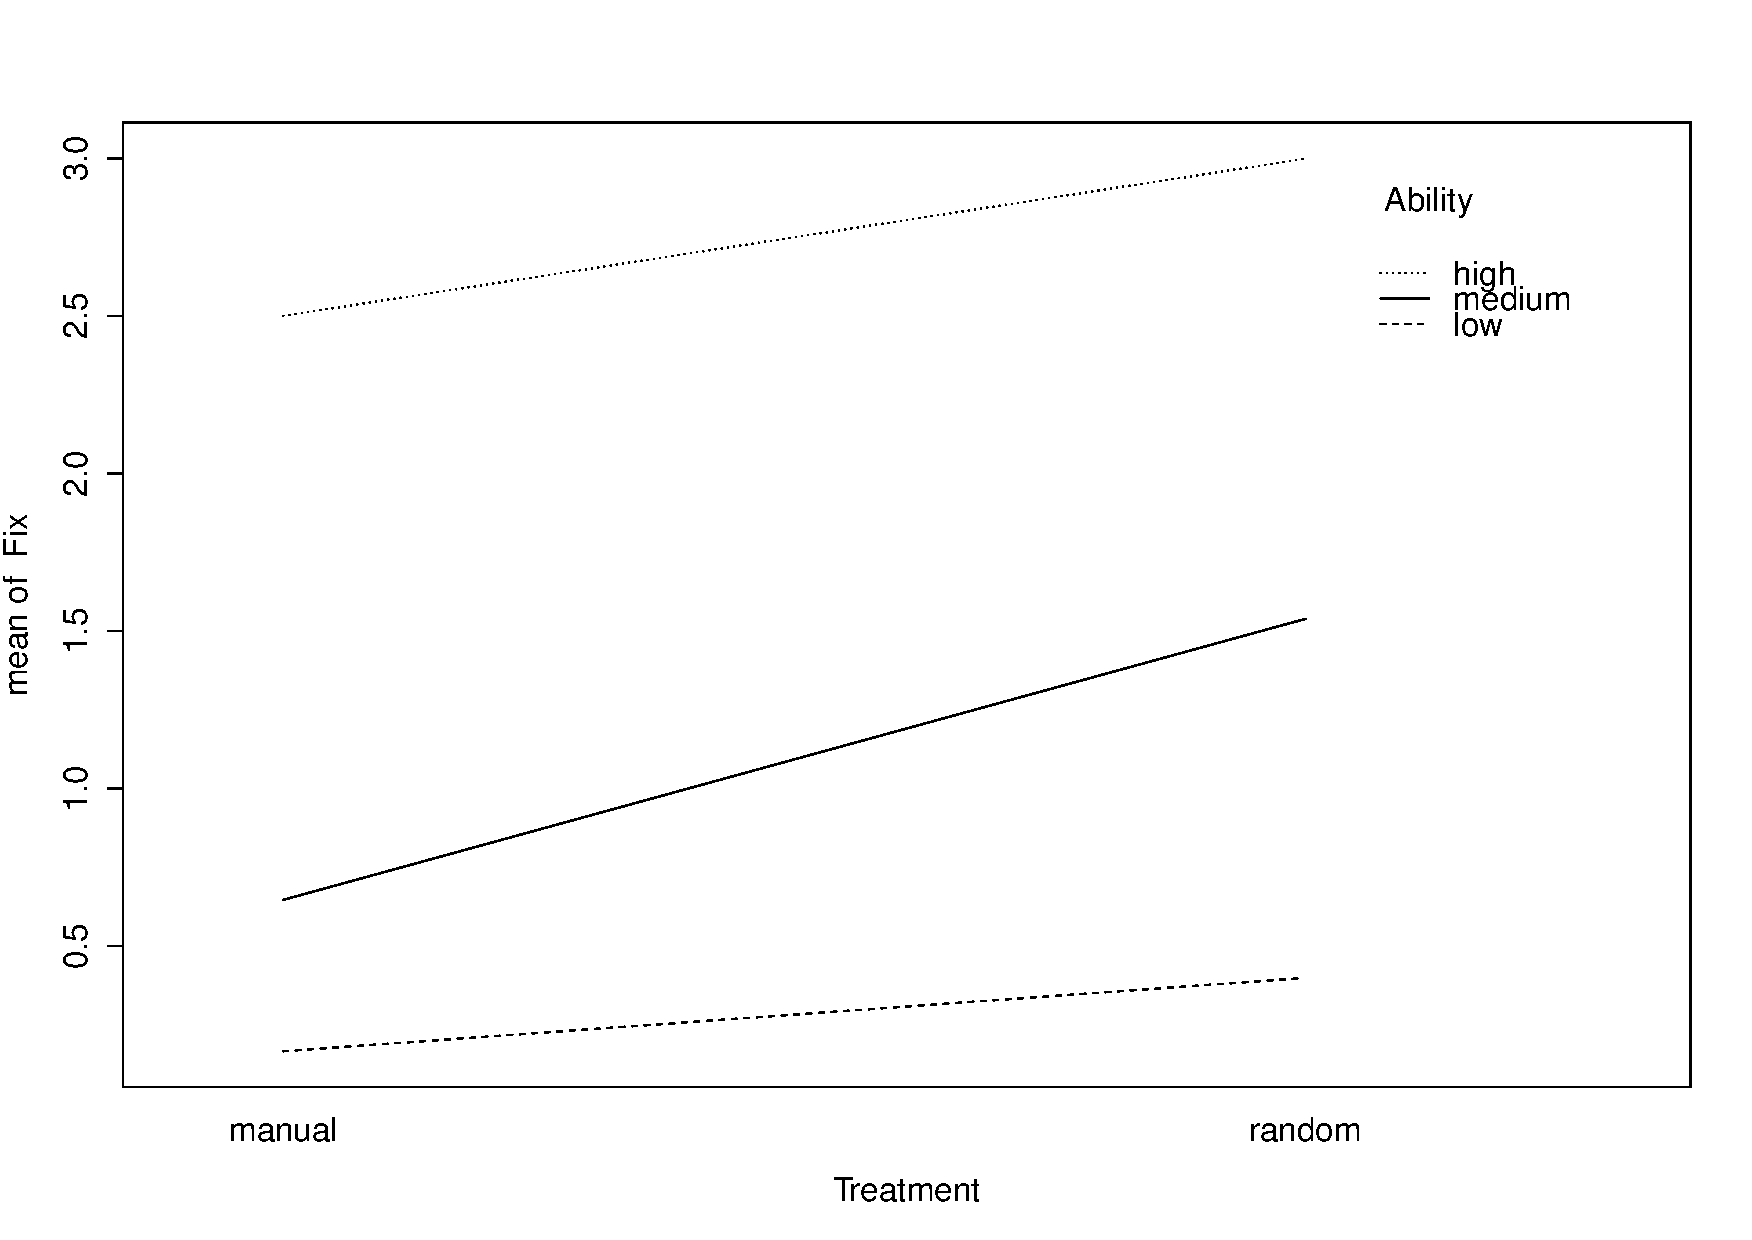
\includegraphics[ width=1 \linewidth]{./img/interaction_FixTreatmentAbility.pdf}
	\caption{Treatment, Effectiveness and Ability Interaction plot}
	\label{int_fix}
\end{figure}

Report conclusion about effectiveness can be summarized in the following quotation:
\begin{quote}
	\begin{itemize}
	\itembf{Treatment:} We can observe that subjects who used autogen tests showed better effectiveness (i.e., correctly fixed more faults) than subjects who used manually written tests.
	
	\itembf{Ability:} We can notice that the high ability and high experience subjects are associated with a line substantially higher than the line for the low ability/experience subjects
	
	\itembf{Experience:} high experience subjects improve their performance when using autogen tests much more than lower experience subjects do. In other words, subjects with high experience are better at taking advantage of the higher effectiveness provided by autogen tests.
	
	\itembf{System and Lab:} we can notice that System and Lab are not significant factors, thus there is no effect
	of the system and no learning effect between the two experimental sessions.
	TREATEMENT: We can observe that subjects who used autogen tests showed better effectiveness (i.e., correctly fixed more faults) than subjects who used manually written tests.

	\end{itemize}
\end{quote}
Accordingly with results we can observe from R output that Efficiency is significantly influenced by Treatment (confidence at 95 \%), Experience (confidence at 95 \%) and Ability (confidence over 99 \%). Session and the System used do not influence Effectiveness in a significant measure. Observing the figure \ref{int_fix} can be seen that all programmers perform better with random test cases, in particular those with medium or higher experience and this is confirmed also from figure \ref{box_fix_treatment}.\\
Experience is also important as can be seen both from figure  \ref{box_fix_ability} and \ref{int_fix}

\subsubsection{Formula}
\begin{equation}
\begin{split}
	\hat{Fix} = f(Tr, Ex, Ab) = A_{1}*Tr + A_{2}*Ex + A_{3}*Ab + A_{0} \\
	\hat{Fix} = f(Tr, Ex, Ab) = 0.696*Tr + 0.77*Ex + 0.944*Ab + -1.396
\end{split}
\end{equation}

% % % % % % % % % % % % % % % % % % % % % % % % % % % % % % % % % % % % % % % % % % % % % % % % % % % % % % % % % % % % % % % % % % % % % % % % % % % % % % % % % % % % % % % % % % % % % % % % % % % % % % % % %
\newpage
\subsection{Efficiency Results}
This is the raw data output of the efficiency experiment's GLM.
\begin{lstlisting}[language=]
Call:
glm(formula = Efficiency ~ System + Treatment + Lab + Experience + 
    Ability)

Deviance Residuals: 
      Min         1Q     Median         3Q        Max  
-0.061021  -0.021901  -0.009289   0.017966   0.203006  

Coefficients:
                     Estimate Std. Error t value Pr(>|t|)    
(Intercept)        -0.0784003  0.0232811  -3.368  0.00158 ** 
Systemxml-security -0.0103287  0.0131413  -0.786  0.43610    
Treatmentrandom     0.0408678  0.0130782   3.125  0.00315 ** 
Lablab2             0.0005354  0.0134652   0.040  0.96847    
Experiencemsc       0.0208320  0.0137561   1.514  0.13708    
Ability             0.0490092  0.0111127   4.410 6.57e-05 ***
---
Signif. codes:  0 ‘***’ 0.001 ‘**’ 0.01 ‘*’ 0.05 ‘.’ 0.1 ‘ ’ 1

(Dispersion parameter for gaussian family taken to be 0.002103959)

    Null deviance: 0.183689  on 49  degrees of freedom
Residual deviance: 0.092574  on 44  degrees of freedom
AIC: -158.69

Number of Fisher Scoring iterations: 2
\end{lstlisting}

\begin{figure}
		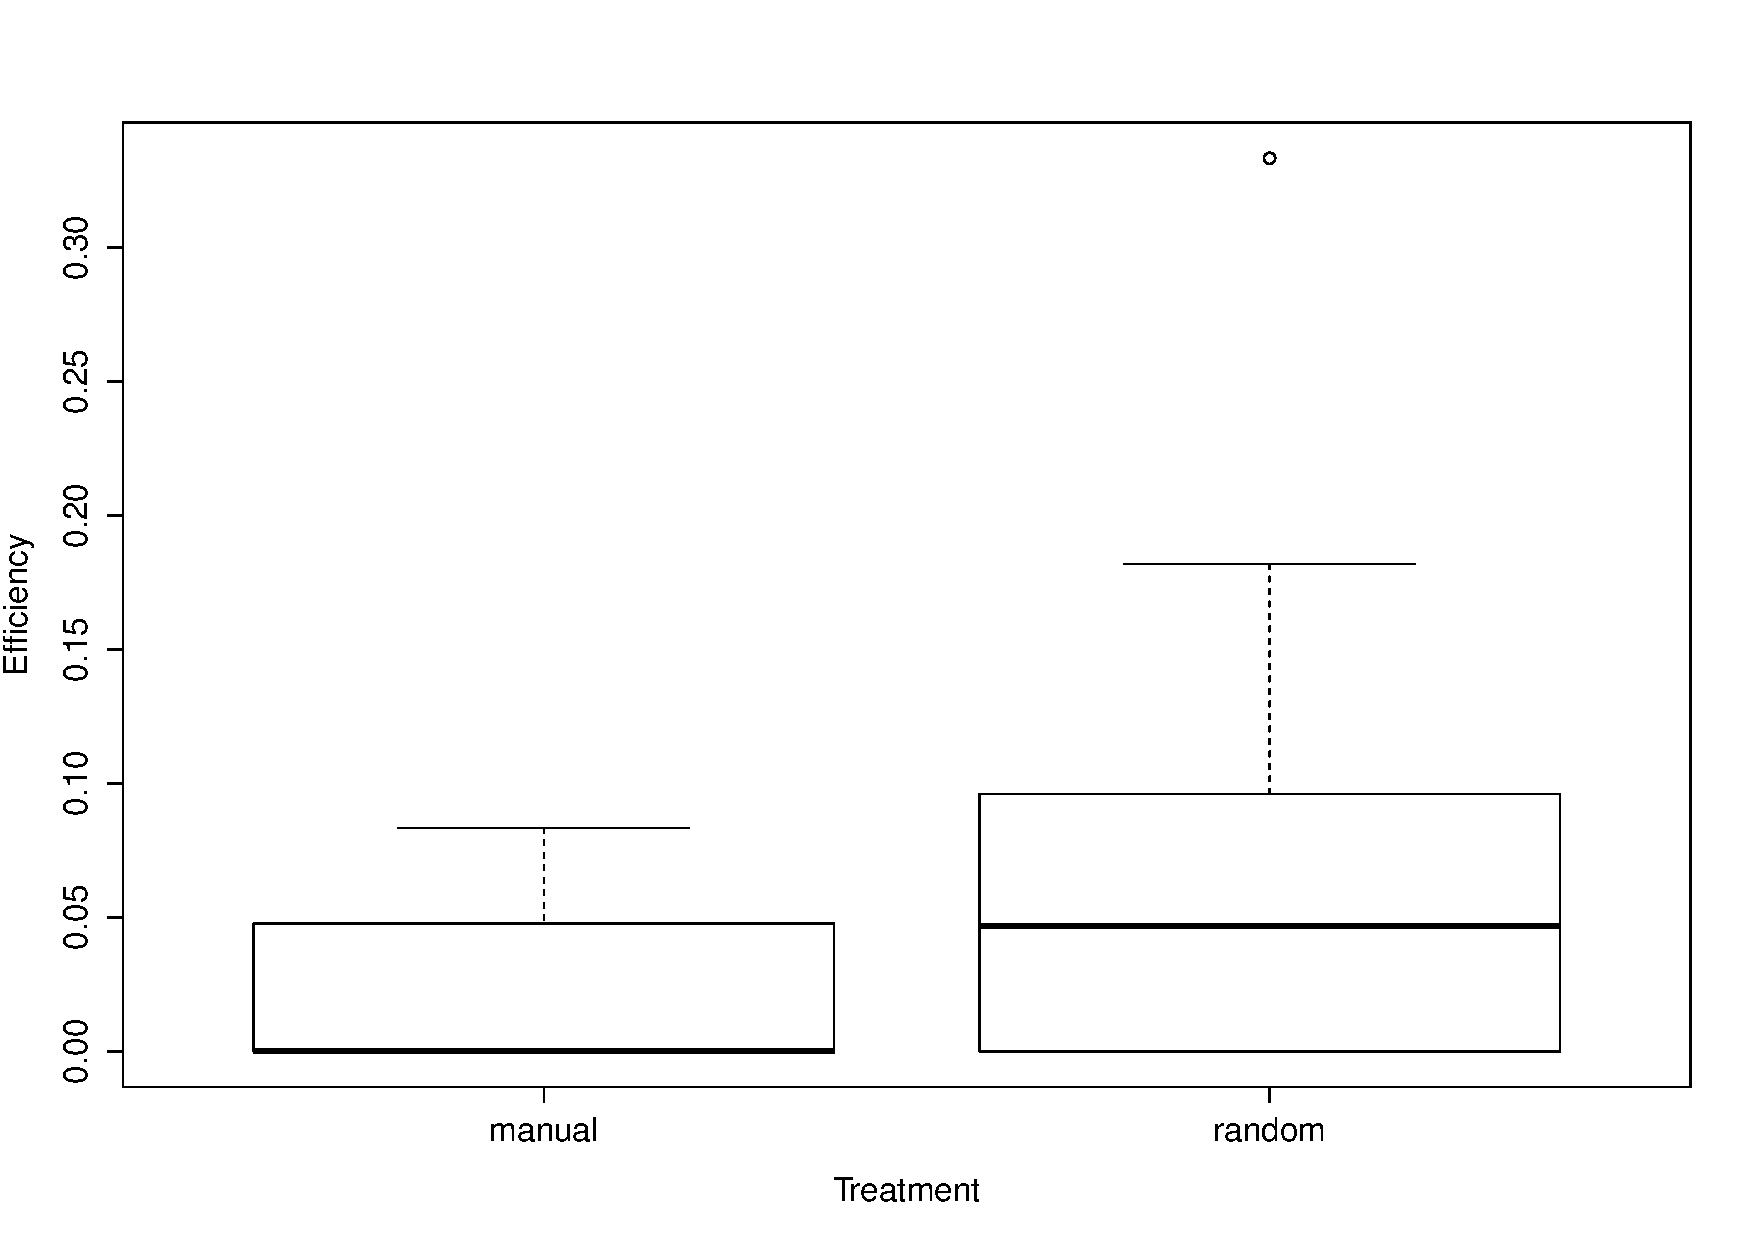
\includegraphics[ width=0.5 \linewidth]{./img/box_eff_treatment.pdf}
		\caption{Efficiency-Treatment Boxplot}
		\label{box_eff_treatment}\begin{equation}
		\begin{split}
			\hat{Fix} = f(Tr, Ex, Ab) = A_{1}*Tr + A_{2}*Ex + A_{3}*Ab + A_{0} \\
			\hat{Fix} = f(Tr, Ex, Ab) = 0.696*Tr + 0.77*Ex + 0.944*Ab + -1.396
		\end{split}
		\end{equation}
	\end{figure}

\begin{figure}
	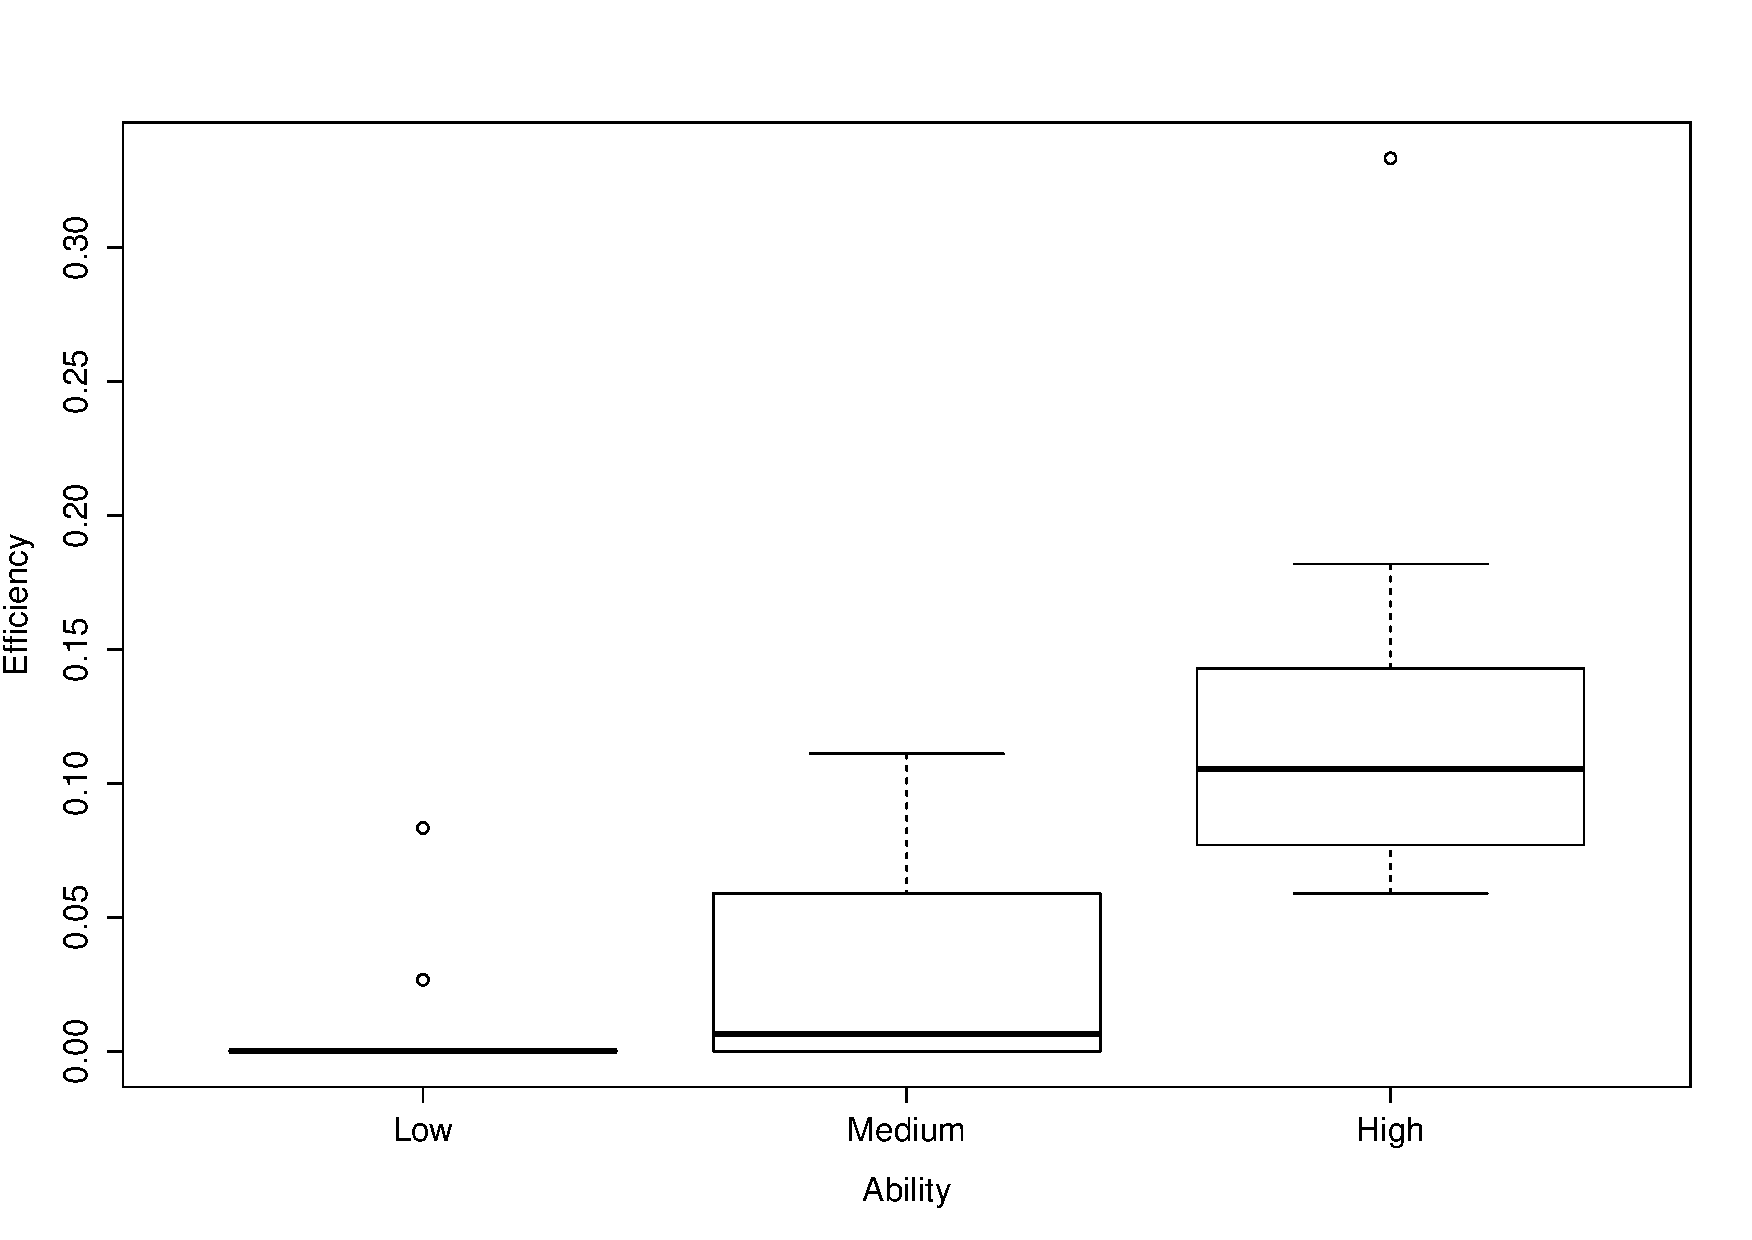
\includegraphics[ width=0.5 \linewidth]{./img/box_eff_ability.pdf}
	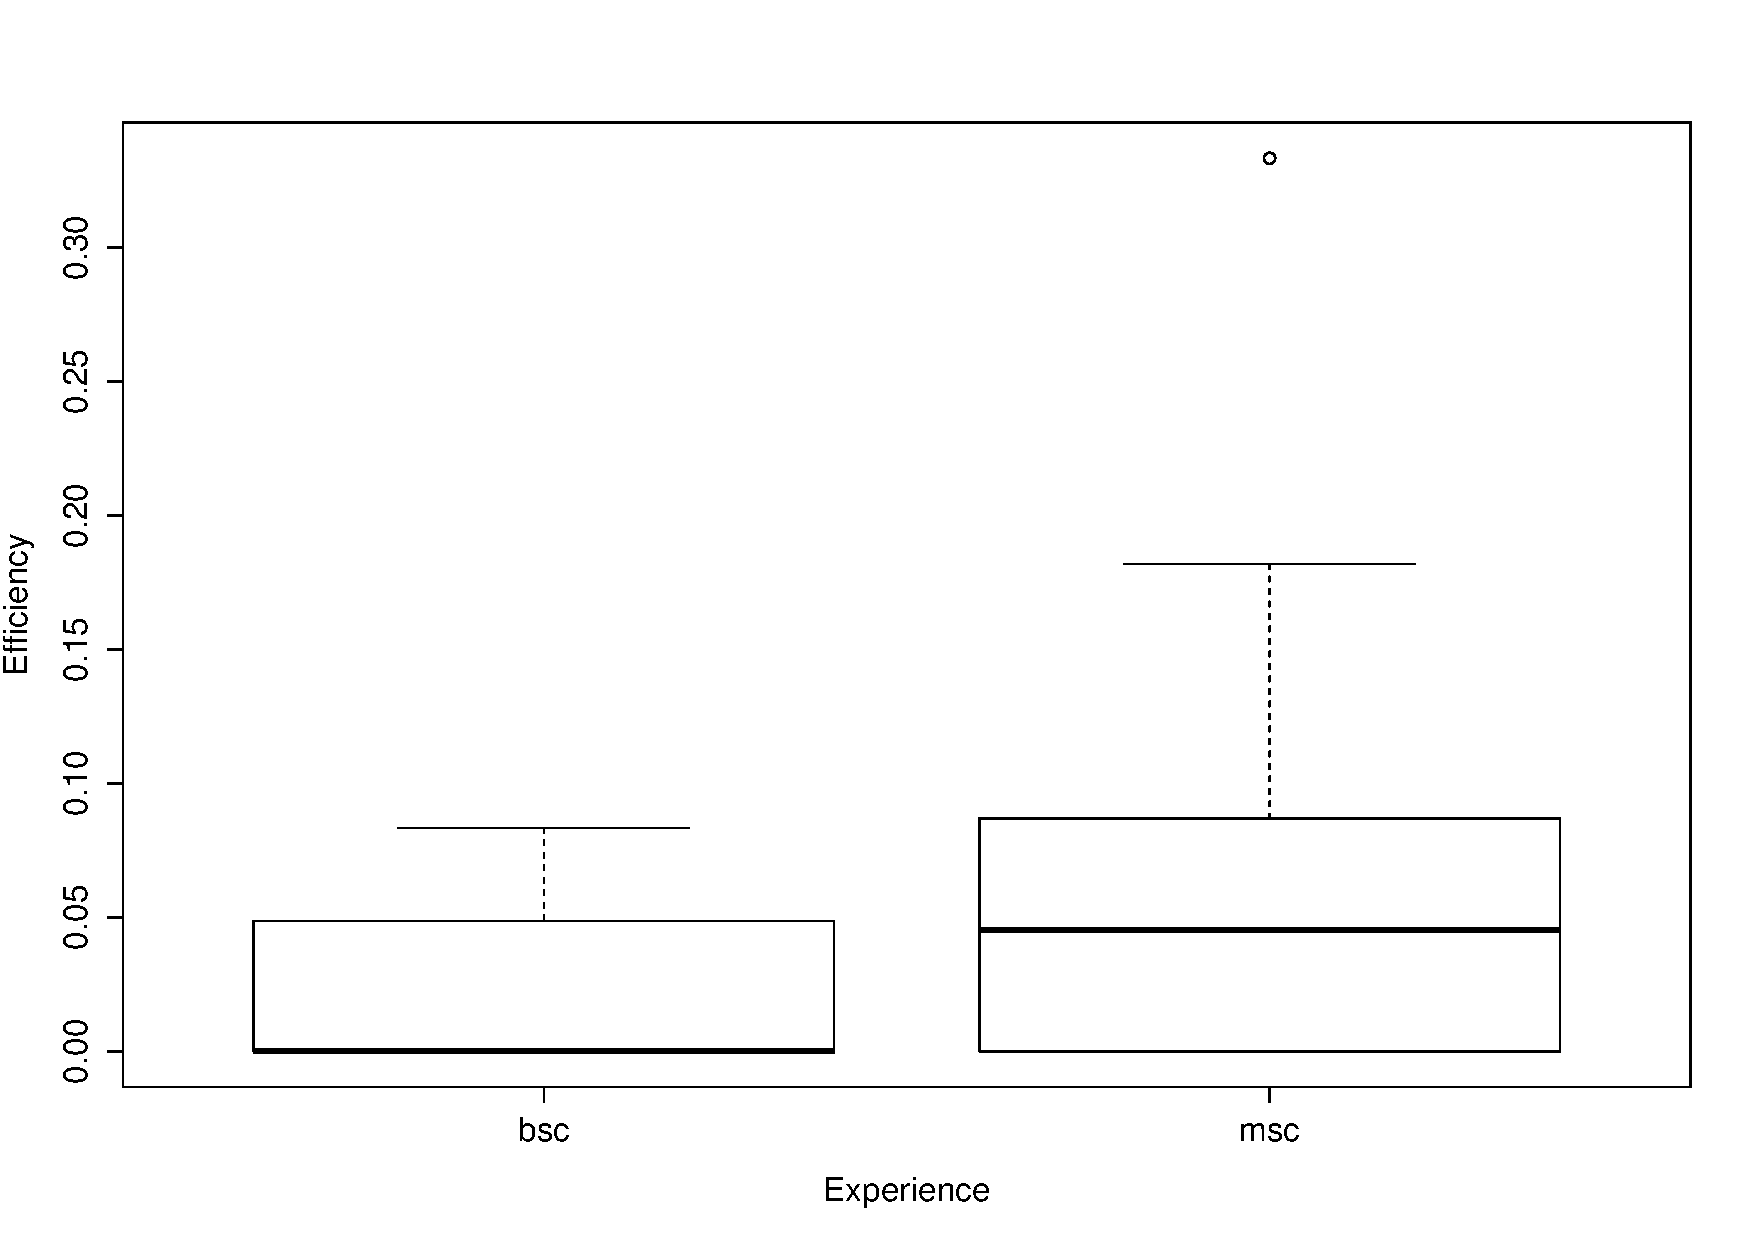
\includegraphics[ width=0.5 \linewidth]{./img/box_eff_experience.pdf}
	\caption{Efficiency respect to Ability and experience Boxplots}
	\label{box_eff_ability}
\end{figure}

\begin{figure}
	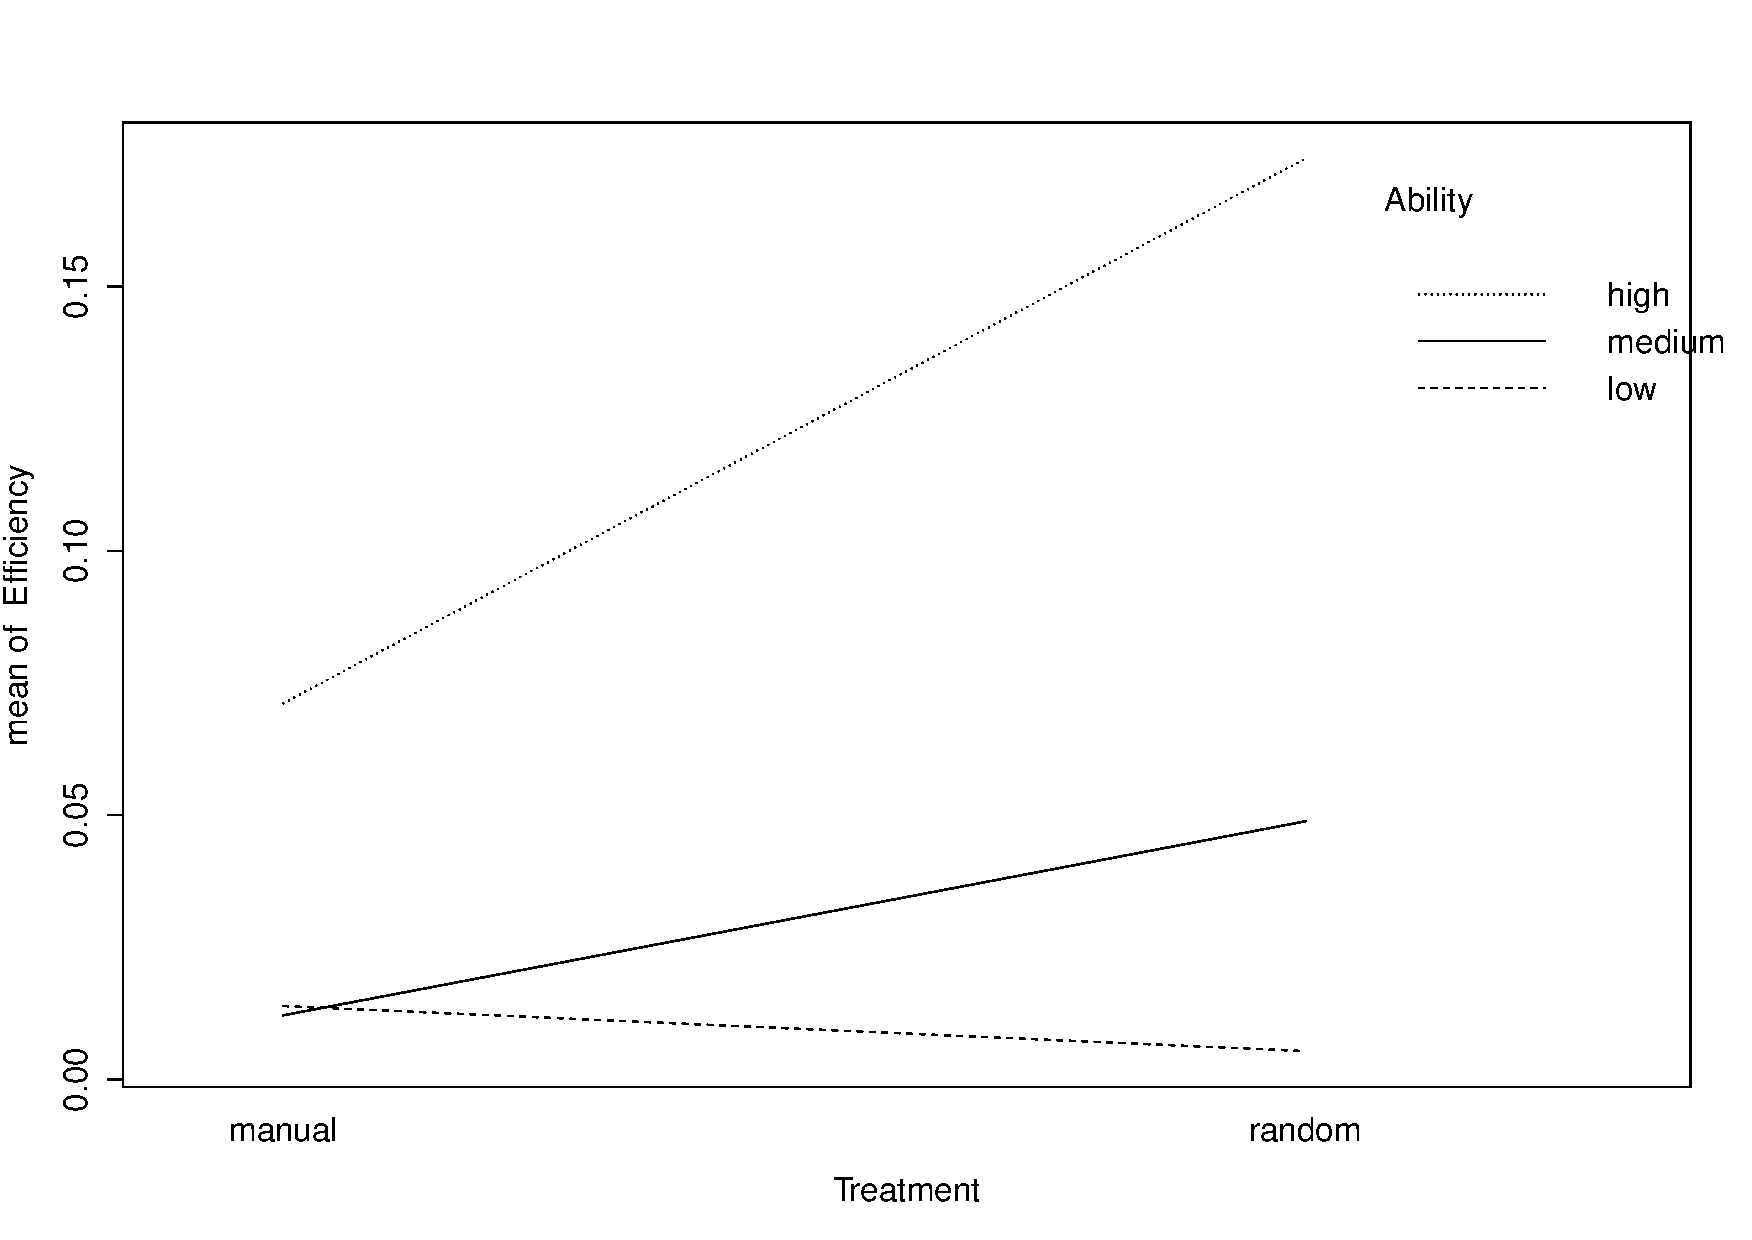
\includegraphics[ width=1 \linewidth]{./img/interaction_EfficiencyTreatmentAbility.pdf}
	\caption{Treatment, Efficiency and Ability Interaction plot}
	\label{int_eff}
\end{figure}

Report conclusion about effectiveness can be summarized in the following quotation:
\begin{quote}
	\begin{itemize}
	\itembf{Treatment:} The efficiency of subjects working with autogen tests is higher than when working with manually	written tests.  
	
	\itembf{Ability and Experience:} Higher ability/experience subjects are particularly	good at taking advantage of the higher efficiency associated with the use of autogen tests.
	
	\itembf{System and Lab:} Factors System and Lab do not have a significant influence on efficiency of debugging.
	of the system and no learning effect between the two experimental sessions.

	\end{itemize}
\end{quote}
Accordingly with results we can observe from R output that Efficiency is significantly influenced by Treatment (confidence at 99 \%) and Ability (confidence over 99 \%). Nor experience neither Session and the System used influence Efficiency in a significant measure.\\
Observing the figure \ref{int_eff} can be seen that programmers with medium or higher experience performs significantly better with random test while lesser experienced developers performs better with manual test. This strange behavior can be explained looking at data table: most data involving low-ability programmers are corrupted and only two cases are significant, all other rows report a fix and efficiency equal to 0 because of several missing data. This probably also influence Experience result: most low-ability subjects are also bsc.

\subsubsection{Formula}
\begin{equation}
\begin{split}
	\hat{Eff} = f(Tr, Ab) = A_{1}*Tr + A_{2}*Ab + A_{0} \\
	\hat{Eff} = f(Tr, Ab) = 0.04*Tr + 0.049*Ab + -0.078
\end{split}
\end{equation}